\documentclass{uscthesis}

%%%%%%%%%%%%%%%%%%%%%%%%%%%%%%%%%%%%%%%%%%
%%% Options include: [forbinding], which produces 
%%% an alternative title page and an appropriate
%%% binding margin,  [honors] for Honors College theses,
%%% and [durt] for undergraduate thesis submitted as part
%%% part of the distinction in mathematics program.
%%%%%%%%%%%%%%%%%%%%%%%%%%%%%%%%%%%%%%%%%%

%%%%%%%%%%%%%%%%%%%%%%%%%%%%%%%%%%%%%%%%%%
%%  LaTeX Preamble
%%%%%%%%%%%%%%%%%%%%%%%%%%%%%%%%%%%%%%%%%%
\usepackage{graphicx}
\usepackage{amsmath,amsfonts,amssymb}
\usepackage[version=4]{mhchem} % Formula subscripts using \ce{}
\usepackage{tikz}
\usepackage{upgreek}
\usepackage{lscape}
\usepackage{lineno}
% \usepackage{caption}
\usepackage[position=t,singlelinecheck=off]{subfig}
\usepackage{cleveref}
\usepackage
%[disable]
{todonotes}
\usepackage{siunitx}
\usepackage[section]{placeins}
\usepackage[english]{babel}


%%%%%%%%%%%%%%%%%%%%%%%%%%%%%%%%%%%%%%%%%%
%% You should include above
%% any LaTeX packages that you need.  Most packages should work 
%% with this documentclass.
%%%%%%%%%%%%%%%%%%%%%%%%%%%%%%%%%%%%%%%%%

\bibliographystyle{amsplain}

%%%%%%%%%%%%%%%%%%%%%%%%%%%%%%%%%%%%%%%%
%% The lines above specify a BibTeX style which controls 
%% the appearance of the bibliography and how citations to
%% the bibliography within the text will work.  It is based on the biblatex.sty
%% package and provides a Chicago style, as preferred by the Graduate School.
%% There are other acceptable styles.  Indeed, different academic disciplines
%% have different styles.
%% 
%% The line  \bibliography{references} will cause LaTeX is search for a file
%% called thesis.bib.  This file could be named differently.  For example
%% \bibliography{henry} would provoke a search for henry.bib.  The
%% file reference.bib (or henry.bib) is one you will have to produce.  It is
%% a BibTeX database of references you use.
%% 
%% There are a number of alternate ways to address your bibliographic needs.
%% See the documentation uscthesisdoc.pdf  for a discussion of the different options.
%%
%%
%% 
%%In any case, this  is a good spot to ask LaTeX to load what it needs to handle
%% literature citations and to layout the bibliography. 
%%
%%%%%%%%%%%%%%%%%%%%%%%%%%%%%%%%%%%%%%%%%%


\newtheorem{thm}{Theorem}[chapter]
\newtheorem*{thmun}{Theorem}
\newtheorem{cor}[thm]{Corollary}
\newtheorem{lem}[thm]{Lemma}
\theoremstyle{definition}
\newtheorem{defn}[thm]{Definition}
\newtheorem{ex}[thm]{Example}
\theoremstyle{plain}

\tikzset{>=stealth}
\usetikzlibrary{positioning}

%%%%%%%%%%%%%%%%%%%%%%%%%%%%%%%%%%%%%%%%%%%%
%%  These are just a few sample lines. Put here any 
%%  commands of your own devising that you want to use.
%%  If these examples are no use to you, omit them.
%%%%%%%%%%%%%%%%%%%%%%%%%%%%%%%%%%%%%%%%%%%%%

\newcommand{\grad}[1]{\vec{\nabla} #1} % for gradient
\newcommand{\iA}{\AA$^{-1}$}
\setcounter{tocdepth}{4}
\setcounter{secnumdepth}{4}

%%%%%%%%%%%%%%%%%%%%%%%%%%%%%%%%%%%%%%%%%%%%%%%%%%%%%%
%%             The Front Matter
%%  The section below deals with the material that comes 
%%  before the actual content of the document: The title 
%%  page, abstract, acknowledgments,etc.
%%
%%  Some of it is required.
%%%%%%%%%%%%%%%%%%%%%%%%%%%%%%%%%%%%%%%%%%%%%%%%%%%%%%

\title{Solving Atomic Structures using Statistical Mechanical Searches on X-ray Scattering Derived Potential Energy Surfaces}

\author{Christopher James}{Wright}    %% First Name then 
                                 %% Last Name

\date{2016}                      %% The year of graduation

\otherdegrees{
Bachelor of Science\\
Brown University 2014\\ [\baselineskip]
%% The \\ on this line is 
}                                %% ESSENTIAL!

\degree{Masters of Science}     %% The Graduate School provides 
                                 %% a list of official degrees.
\field{Chemical Engineering}              %% Fields also provided by the 
                                 %% Graduate School.
\college{College of Engineering and Computing}  %%As listed by Grad School

\advisor {Dr.}{Xiao-Dong Zhou}{Major Professor}  %%% Be sure the 
\readera{Dr.}{Mark Uline}{Committee Member}          %%% the one used in 
\readerb{Dr.}{Jochen Lauterbach}{Committee Member} %%% your department.
% \readerc{Dr.}{Thomas Vogt}{Committee Member}     %%% third field is %%% If you have just two readers, for example, leave out \readerc and
%%% \readerd
%%%
%%% For Honors College theses use \reader{}{}   NO third field.
%%% The commands \otherdegrees, \degree, \field, \college, \readera, etc.
%%% are not used under the honors option.
%%%%%%%%%%%%%%%%%%%%%%%%%%%%%%%%%%%%%%%%%%%%%%%%%%%%%%%

\dean{Lacy Ford}   %% The Dean of the Graduate School
                   %% BE SURE TO CHECK THE NAME OF THE
                   %%PERSON CURRENTLY HOLDING THIS POSITION
                     %% For Honors College theses use
                     %% \schcsigner{}{}.  For example,
                     %% \schcsigner{Dr.}{Davis Baird}

\copyrightpage       %% This is optional. It makes a 
                     %% copyright page that will appear 
                     %% immediately after the title page.

\abstract{misc/abstract}  %% This calls the file herkimer.tex but
                     %% but you might replace herkimer by 
                     %% anything you like, for example by 
                     %% abstract. Note, the Graduate School
                     %% REQUIRES that PhD dissertations have 
                     %% abstracts.
                     %%
                     %% For Honors College theses use
                     %% \honorsabstract{}


\acknowledgments{misc/thanks} %% This calls the file thanks.tex 
%% This is optional       %% where you have put your 
                          %%acknowledgments.

\dedication{misc/dedication}   %% Calls dedication.tex
%%% Also optional

% \preface{forward}    %% Calls forward.tex.  Optional.

\makeLoT               %% Issue this command if your work has 
                       %% four or more tables.  A list of tables 
                       %% will be produced automatically.

\makeLoF               %% works the same way but for figures.

%%%%%%%%%%%%%%%%%%%%%%%%%%%%%%%%%%%%%%%%%%%%%%%%%%%%%%%%%%%%
%%  Finally, here is the meat.  The idea is to compose a 
%%  .tex file for each section of your thesis or dissertation.  
%%  Then use LaTeX's \include command to put them all together.  
%%  Doing it this way makes it easier to change the order of 
%%  exposition as your writing is in progress.  Also it
%%  makes it easy to print out just one section. The \include
%%  command always starts a new page. So every section would 
%%  start on a new page.  If you would like for sections just
%%  to continue, after the appropriate vertical space, on the
%%  current page, then use the \input command instead of the 
%%  \include command.
%%%%%%%%%%%%%%%%%%%%%%%%%%%%%%%%%%%%%%%%%%%%%%%%%%%%%%%%%%%%

\begin{document}
\linenumbers
\todototoc
\listoftodos
\todo[inline]{Need more references}
\chapter*{Introduction} \label{intro}
Engineering materials and chemicals on the atomic scale has long been a goal for the chemistry, physics, materials science, and chemical engineering fields.
Realizing this goal could lead to durable fuel cell catalysts, more bioavailable pharmaceuticals, and radiation damage resistant spacecraft shielding.
Before we can even think of making atomistically exact structures, durable structures, or structures which change in reproducible ways, we need to know the atomic structure exactly.
This work addresses these issues by developing a methodology for solving the structure of nanomaterials by matching experimental x-ray scattering data with simulated atomic structures.

Chapter \ref{ch:pes_e} develops the statistical mechanical system used to match the theoretical structure.
\S \ref{sec:pes} focuses on the development of potential energy surfaces, including potential energy and force equations, which have minima where experimental results and simulated structures agree the most.
\S \ref{sec:ens} will discuss statistical mechanical ensembles which are used to search for minima on the potential energy surface.

Chapter \ref{ch:pdf} will discuss the mathematical and computational development of the atomic pair distribution function (PDF).
\S \ref{sec:comp} will focus on the rapid graphical processing unit based calculation of the PDF and its gradients.

Chapter \ref{ch:bmk} will discuss the benchmarking of the the combined statistical mechanical optimizer and PDF calculation systems against a series of theoretical nanoparticles, focusing on understanding limitations of the method and structure reproduction.

Chapter \ref{ch:dp} will focus on the acquisition of experimental data, its management, and processing.
\S \ref{subsec:qres}, \ref{subsec:mask}, and \ref{subsec:int} will discuss the derivation of the $Q$ resolution function, the automated masking of 2D area detectors for x-ray total scattering measurements using the previously derived $Q$ resolution, and the impact of different averaging methods and masks on azimuthal integration, respectively.

Chapter \ref{ch:pno} will discuss preliminary experimental results investigating the phase changes and local structure of \ce{Pr2NiO4}    %% Calls Introduction.tex
                          %% Honors theses are required to 
                          %% have an Introduction.  For
                          %% Honors theses, the file 
                          %% Introduction.tex should begin
                          %%
                          %% \chapter*{Introduction}
                          %% followed by the text of the 
                          %% introduction.


\chapter{Statistical Mechanical Ensembles and Potential Energy Surfaces} \label{ch:pes_e}
\section{Introduction}
The approach taken in this work for solving the atomic structures of materials is one of optimization.
The plan is to develop a potential energy surface (PES) which has minima associated with atomic structures who's properties match the experimentally observed properties.
Thus, the various positional variables of the structure can be solved by optimizing the structure against the PES.
This approach is popular in the PDF community for solving the structure of materials using both extensive large box models and simpler small box models.

In this chapter we discuss the development of the various PESs used in the PDF community for comparing theoretical and experimental PDFs.
Special attention will be paid to the gradients of the potential energy functions, as these are important to some optimization techniques.
Additionally, we also discuss the use of statistical mechanical ensembles for finding minima on the PES.

\section{Potential Energy Surfaces} \label{sec:pes}
A PES simply describes the potential energy of the system as a function of all its relevent coordinates in phase space, essentially providing a mapping $\mathbb{R}^{n} \rightarrow \mathbb{R}$, where $\mathbb{R}$ is the set of real numbers and $n$ is the number of positional parameters in the system.
Usually these coordinates are the positions of the atoms $q$ and their conjugate the momenta $p$.
Note that there could be more variables associated with the system, for instance the magnetic moments of the atoms could play a role in describing the system.
In this magnetic system there would be positional variables for the atomwise spin vectors and their "momenta".
Application of the term "momenta" might seem odd here, as the magnetic spin does not have a mass or a velocity.
However, since the magnetic "position" is defined on the PES we need to describe its conjugate varible to properly formulate Hamitonian dynamics and the kinetic portion of the PES.

\subsection{Experimentally Derived Potential Energy Surfaces}
Generally PESs are obtained from purely computational experiments including: ab-initio DFT, classical approximations via the embedded atom method, or even parameter driven models with experimentally fitted parameters.
However, one can dervive a PES from an experiment which describes how well the model reproduces the experimental data.
In this case one needs a theoretical and computational framework mapping the atomistic variables of the simulation to the same space of the data obtained from the experiment.
This allows the experiment to be compared directly against the predicted data via an experimentally derived PES.
\subsubsection{Potentials}
For an experiment which produces 1D data, like powder diffraction, EXAFS or XPS, the implemented potentials are:
\begin{equation} \label{chi}
\chi^{2} =
\sum_{a=a_\mathrm{min}}^{a_\mathrm{max}} \left(A_{_\mathrm{obs}} - \alpha A_{_\mathrm{calc}}\right)^{2}
\end{equation}
\begin{equation}\label{Rw}
Rw =
\sqrt{\frac{\sum_{a=a_\mathrm{min}}^{a_\mathrm{max}} \left(A_{_\mathrm{obs}} - \alpha A_{_\mathrm{calc}}\right)^{2}}{\sum_{a=a_\mathrm{min}}^{a_\mathrm{max}} A_{_\mathrm{obs}}^{2}}}
\end{equation}
\begin{equation}\label{INVERT}
  \chi^{2}_{\mathrm{INVERT}} = \frac{1}{N}\sum_{j}\sum_{r}[A_{obs}(r) - \alpha A_{j_\mathrm{calc}}(r)]^{2}
\end{equation}
\begin{equation} \label{alpha}
\alpha  = \frac{\sum_{a=a_\mathrm{min}}^{a_\mathrm{max}}A_\mathrm{_\mathrm{obs}}A_{_\mathrm{calc}}}{\sum_{a=a_\mathrm{min}}^{a_\mathrm{max}} A_{_\mathrm{calc}}^{2}} = \frac{\vec{A}_{_\mathrm{obs}}\cdot\vec{A}_\mathrm{calc}}{|\vec{A}_\mathrm{calc}|^{2}}
\end{equation}
where $A_{calc}$ and $A_{obs}$ are the calculated and observed 1D experimental data
and $A_{calc, j}$ is the calculated data for a single atom interacting with the other atoms of the system.
Note that $A_{calc}$ has a dependence on $q$, the positions of the system.

The $Rw$ and $\chi^{2}$ potentials have been reported numerous times. \cite{Petkov2014, Masadeh2007, Choi2013, McGreevy, Proffen1997}
Essentially these potentials measure the least squares distance between the observed scattering and the predicted scattering poviding a way to quantify the agreement between the model and experiment.
While $RW$ and $\chi^{2}$ are now standard in the PDF community, the $\mathrm{INVERT}$ potential is fairly new and aims to incorperate descriptions of the structural symmetry into the PES. \cite{Cliffe2010, Cliffe2013}
In the case of the $\mathrm{INVERT}$ potential NMR or other symmetry sensitive data is used to describe the number of unique atomic coordinations.
This is then used to describe the number of unique atomwise pair distribution functions, thus causing systems with more or less unique coordination environments to be higher in energy.
This approach has been shown to be useful for \ce{C60} and other systems which are highly symmetric, creating a PES with an easier to find minima. \cite{Cliffe2010, Cliffe2013}
However, many times this kind of data is unavailable when refining the structure causing the potential to be less useful.
Additionally, this potential introduces an element of user bias as the refiner must decide, based on some spectroscopic data, how many unique environments are in the material.
This bias could be removed by using one of the other potentials with a method for simulating the observed spectra, allowing the computational system decide what structures properly reproduce all the observed data.

\subsubsection{Forces}
\begin{equation}
\grad{\chi^{2}} =
- 2 \sum_{a=a_\mathrm{min}}^{a_\mathrm{max}} (\alpha \frac{\partial A_{_\mathrm{calc}}}{\partial \gamma_{i, w}} + A_{_\mathrm{calc}} \frac{\partial \alpha}{\partial \gamma_{i, w}} ) (A_{_\mathrm{obs}} - \alpha A_{_\mathrm{calc}})
\end{equation}
\begin{equation}
\grad{Rw} =
\frac{Rw}{\chi^{2}} \sum_{a=a_\mathrm{min}}^{a_\mathrm{max}} (\alpha \frac{\partial A_{_\mathrm{calc}}}{\partial \gamma_{i, w}} + A_{_\mathrm{calc}} \frac{\partial \alpha}{\partial \gamma_{i, w}} ) (\alpha A_{_\mathrm{calc}}  - (A_{_\mathrm{obs}}))
\end{equation}
\begin{equation}
  \grad{\chi^{2}_{\mathrm{INVERT}}} = \frac{-2}{N} \sum_{a=a_\mathrm{min}}^{a_\mathrm{max}} \sum_{j}(\alpha \frac{\partial A_{j_\mathrm{calc}}}{\partial \gamma_{i, w}} + A_{j_\mathrm{calc}} \frac{\partial \alpha}{\partial \gamma_{i, w}} ) (A_{_\mathrm{obs}} - \alpha A_{j_\mathrm{calc}})
\end{equation}
\begin{equation}
\frac{\partial \alpha}{\partial \gamma_{i, w}}  =
\frac{(\sum_{a=a_\mathrm{min}}^{a_\mathrm{max}} A_{_\mathrm{obs}} \frac{\partial A_{_\mathrm{calc}}}{\partial \gamma_{i, w}}- 2\alpha \sum_{a=a_\mathrm{min}}^{a_\mathrm{max}} A_{_\mathrm{calc}} \frac{\partial A_{_\mathrm{calc}}}{\partial \gamma_{i, w}})}{\sum_{a=a_\mathrm{min}}^{a_\mathrm{max}} A_{_\mathrm{calc}}^{2}}
\end{equation}
where $\gamma_{i, w}$ is the $i$th arbitrary positional variable in the $w$th direction.
The concept of an "arbitrary positional variable" might seem a bit cumbersome but it allows us to define the forces for any atomic parameter which can be represented as a vector in 3-space.
This comes in handy when trying to define the forces acting on variables like anistropic displacement parameters or atomic magnetic spins.

\graphicspath{{./pes_e/figures/}}
\section{Ensembles} \label{sec:ens}
While PESs describe which atomic configurations are the most desirable and how the atoms would like to get there, the ensemble describes how the atoms move on the PES.
The abstraction of the PES from the ensemble is an important one, as it allows for the reuse and exchange of both PESs and ensembles for a wide array of problems.
Statistical mechanical ensembles can be described in two ways, analytically and scholastically.
For long simulation times and fine enough numerical or analytical integration these two descriptions should be identical.

In either case one starts by defining the Hamiltonian, $\mathcal{H}$, as the total energy of the system.
Thus, the Hamiltonian is described as the sum of the potential $U(q)$ and kinetic $K(p)$ energies, where $q$ is the positions of the atoms and $p$ is their momenta
\begin{equation} \label{Hamiltonian}
  \mathcal{H}(q, p) = U(q) + K(p)
\end{equation}
\noindent where $K(p) = \frac{1}{2}\sum_{i} \frac{p_{i}^{2}}{m_{i}}$ and $i$ denotes the $i$th particle.

Analytically one generally defines a partition function, which describes the sum of probabilities over all potential atomic states.
\begin{equation}
\Xi = \sum_{i} P_{i}(q, p)
\end{equation}
where $P_{i}$ is the probability of the $i$th state and is a function of the total energy of that state.
This partition function can then be used to obtain the probability of any specific state.
The relationship of the probability of a state to the state's energy and other properties depends on the ensemble being used.
%\begin{equation}
%P(q, p) = \frac{\delta(E - \mathcal{H}(q, p))}{W}
%\end{equation}
%where $E$ is the energy of the system, W is the total number of states in the system, and $\delta$ is the Dirac Delta Function.

For the canonical ensemble the partition function is probability is:
\begin{equation}
Q(N, V, T) = \exp(\frac{-\mathcal{H}(q, p)}{k_{b}T})
\end{equation}
where $k_{b}$ is the Boltzmann constant and $T$ is the temperature of the system. \cite{McQuarrie2000}

\subsection{Monte Carlo Modeling}
Monte Carlo can be used to simulate a statistical mechanical ensemble which can not be solved analytically.
In most Monte Carlo systems the ensemble is simulated by randomly changing one of the system parameters and comparing the energy of the new system against the energy of the old system.
If the energy of the new system is lower than the current energy then the new configuration is accepted.
Otherwise the new system is rejected unless
\begin{equation}
\exp(\frac{-\Delta E}{E_{T}}) < u
\end{equation}
where u is a random number $[0, 1)$ and $E_{T}$ is the thermal energy characteristic to the system.
The ability of Monte Carlo modeling to accept ``bad'' moves allows the system to hop out of local energy minima during the search for the global minimum.
Reverse Monte Carlo (RMC) is similar to Monte Carlo except it uses $\chi^{2}$ as the PES.\cite{McGreevy}

Despite the utility of RMC, and its wide use in the x-ray scattering community, as Hoffman and Gelman state ``Not all MCMC [Markov Chain Monte Carlo] algorithms are created equal''.\cite{Hoffman2014}
RMC, similar to standard Monte Carlo simulations, samples from the PES at random, usually by translating atoms in the system randomly.
This creates a less efficient, random walk based, exploration of the PES.\cite{Hoffman2014, Neal1993}
Thus, methods for suppressing this random walk nature, while still searching the potential energy surface fully are needed.

\subsection{Hamiltonian Monte Carlo}
Hybrid or Hamiltonian Monte Carlo (HMC) can help to address some of these issues.
HMC was developed originally in the lattice quantum chromodynamics community and provides a more efficient, more scalable approach to PES sampling for Monte Carlo.\cite{Duane1987216, Neal2011}
In HMC the PES is explored using Hamiltonian dynamics, essentially following the gradient of the PES to find more acceptable configurations.


In order to model dynamics we need to describe the motion of the particles in our system, thus:
\begin{align}
  \frac{d q_{i}}{d t} &= \frac{\partial \mathcal{H}}{\partial p_{i}} = p_{i}\\
  \frac{d p_{i}}{d t} &= -\frac{\partial \mathcal{H}}{\partial q_{i}} = -\grad{U}
\end{align}
Using these equations we can derive the position and momentum vectors at any point in time using the leap-frog algorithm:
\begin{align}
  p_{i}(t + \delta t/2) &= p_{i}(t) - \frac{\delta t}{2} \frac{\partial }{\partial q_{i}}U(q(t))\\
  q_{i}(t+\delta t)  &= q_{i}(t) + \delta t * p_{i}(t+\delta t/2)\\
  p_{i}(t+\delta t) &=   p_{i}(t + \delta t/2)- \frac{\delta t}{2} \frac{\partial }{\partial q_{i}}U(q(t+\delta t))
\end{align}
Note that $\frac{\partial}{\partial q_{i}}$ is the gradient with respect to $q$ where $i$ denotes the $i$th atom being moved.
Using this notation the gradient is
\begin{equation} \label{grad}
  \grad{U} = \begin{bmatrix}
    \frac{\partial U}{\partial q_{0, x}} & \frac{\partial U}{\partial q_{0, y}} & \frac{\partial U}{\partial q_{0, z}} \\
    \vdots & \frac{\partial U}{\partial q_{i, w}} & \vdots \\
    \frac{\partial U}{\partial q_{n, x}} & \frac{\partial U}{\partial q_{n, y}} & \frac{\partial U}{\partial q_{n, z}} \\
  \end{bmatrix} =
  \begin{bmatrix}
    \vec{\mathcal{F}}_{0} \\
    \vdots \\
    \vec{\mathcal{F}}_{i} \\
    \vdots \\
    \vec{\mathcal{F}}_{n}\\
  \end{bmatrix}
\end{equation}
where $\frac{\partial}{\partial q_{i, w}}$ is the derivative with respect to $q$ where $w$ denotes direction of the derivative ($x$, $y$, or $z$),  $n$ is the number of atoms and $U$ is the potential which depends on $q$, and $\vec{\mathcal{F}_{i}}$ is the "force" on the $i$th atom.
Using these equations new potential configurations are proposed from the PES.
These proposals are checked against the standard Metropolis criteria discussed above, except that the change in potential energy $\Delta E$ is replaced with the change in the Hamiltonian $\Delta \mathcal{H}$.
Note that while this sampling closely simulates the canonical ensemble, it is not exactly the same.
Usually the canonical ensemble is formulated as microcanonical ensembles in contact with an infinite heat bath at a given temperature, or a set of microcanonical ensembles which exchange thermal energy.
However, the HMC ensemble presented here has a momentum bath instead of a temperature bath.
One could imagine the atoms sitting in a simulation box which has walls which can toggle their thermal exchange.
Initially the box starts in the momentum bath, allowing the atoms to come to equilibrium with the bath momentum.
The box is then removed from the bath causing it to become adiabatic.
Hamiltonian dynamics are then propagated inside the box, essentially running a microcanonical simulation.
Once the dynamics are finished the energy of the system is checked with the Metropolis criteria and the box is reintroduced to the momentum bath and the process starts again.

\subsubsection{No-U-Turn Sampling}
Two parameters must be specified in HMC simulations, the step size $\delta$ and the number of steps $N$.
The step size is critical to the stability of the fitting procedure:  with a too small $\delta$ the simulation runs inefficiently producing structures too close to the previous, whereas with a too big $\delta$ the linear approximation for the forces breaks down and often the simulated NP explodes.
The number of steps to take during the dynamics is equally important and an inappropriate choice may result in backtracking or random walk characteristics in the simulations.
In this work, we employ the No-U-Turn Sampling (NUTS) method recently proposed by Hoffman and Gelman to address this issue \cite{Hoffman2014}.
In the NUTS method $\delta$ and $N$ are dynamically computed by examining the ratio of accepted to rejected configurations as well as whether or not the simulation has started to take a U-turn.
The U-Turn criteria makes certain that the simulation stops when it begins to backtrack, preventing excess computation on configurations that have very little new information to offer.
The use of NUTS leaves us with two simulation parameters: the simulation temperature and the target acceptance.
Hoffman and  Gelman have empirically shown that the ideal target acceptance, which governs the dynamics time steps, is .65, which we have used for all of the simulations here.
The simulation temperature sets the magnitude of the random starting momenta for the atoms at the beginning of each dynamics run \cite{Hoffman2014}.

\subsection{Grand Canonical Ensemble}
While NUTS-HMC simulations provide a system to find minima on PESs, the simulation is fundamentally run in the Canonical Ensemble thus the variables in the simulation are limited to a fixed number of particles, simulation volume, and thermal energy.
Fixing the thermal energy and simulation volume is not a problem, as they are not variables of interest in the final structure.
However, specifying the number of atoms in the system can be problematic, as the exact number of atoms in a sample can be difficult to count or a sample could have a distribution of particle sizes.
Thus, a new ensemble needs to be used to allow the number of atoms to vary as a function of the PES.
This new ensemble is the Grand Canonical Ensemble.

\subsubsection{Ensemble description}
In the Grand Canonical Ensemble (GCE) two sets of variables are allowed to change, the atomic positions, and the total number of atoms and their associated identities.
These two variables are controlled by temperature, or average momentum, and chemical potential.
The partition function is
\begin{equation}
  \Xi = \sum_{N=0}^{\infty} Q(N, V, T) \exp{\frac{N\mu\beta}{T}}
\end{equation}
where $Q(N, V, T)$ is the Canonical partition function discussed above, $\mu$ is the chemical potential. \cite{McQuarrie2000}
This is translated into a Monte Carlo system, producing Grand Canonical Monte Carlo (GCMC).
\subsubsection{Grand Canonical Monte Carlo}
While the probabilities for atomic motion are the same as in the Canonical Ensemble, the addition or removal of an atom have their own probabilities. For the addition of an atom the probability is formally:
\begin{equation}
  \min[1, \frac{V}{(N+1) \Lambda(T)^{3}}e^{-\beta\Delta U + \beta \mu}]
\end{equation}
Similarly the removal of an atom has the probability:
\begin{equation}
  \min[1, \frac{(N)\Lambda(T)^{3}}{V}e^{-\beta\Delta U - \beta \mu}]
\end{equation}
However, both of these equations depend of the overall simulation volume and the thermal wavelength, which is undesirable as these are not really properties that we are of interest to these simulations.
Thus, we roll them into the definition of the chemical potential, essentially setting the base chemical potential to counteract these effects.
This makes certain that our simulation does not change if we change the overall cell volume.
A GCMC move consists of creating a new atomic configuration, where an atom has been added or removed, and checking the above criteria.
However, previous results have shown that this method is computationally expensive in dense liquids, and exceedingly expensive in solid materials.
The long simulation times are due to the random nature of the atomic additions or removals which produce: over-tightly packed atoms, atoms in the middle of nowhere, or nonphysical vacancies.
These configurations are rejected by the GCMC criteria but their probability of being sampled is much higher than configurations which are lower in energy, since the number of incorrect ways to add/remove atoms is much larger than the correct ways.
Thus, we have implemented methods for biasing the atomic addition positions and the atomic removals toward configurations which are more likely to be accepted.

\subsubsection{GCMC biasing}
The basic idea of GCMC biasing is mapping, in 3 dimensions, where an atomic addition or removal is most likely to be accepted.
Thus, the simulation volume is broken up into voxels, 3 dimensional volumes which are contained by the total simulation volume, with a pre-set size.
Each voxel is given a probability of being chosen for a trial insertion where the probability is:
\begin{equation}
  P_{i, j, k} = \frac{e^{\beta \Delta U_{i, j, k}}}{\sum_{i, j, k}e^{\beta \Delta U_{i, j, k}}}
\end{equation}
where $\Delta U_{i, j, k}$ is the change in energy.
However, calculating $\Delta U_{i, j, k}$ can be particularly expensive, especially when calculating scattering from atomic positions.
The computational expense can be mitigated by using a cheaper potential, if only for the evaluation of the voxel energy, as previously shown.
Similar to previous work we can use the Lennard Jones potential to approximate the addition potential, lowering the computational burden. \cite{Snurr1993}

Atomic deletion follows a similar biasing procedure, calculating the energy of each atom and biasing the probability of each atom to be chosen for removal by its energy.
This way atoms which add the most energy to the system are more likely to be removed.

\begin{figure}
    \centering
    \subfloat[]{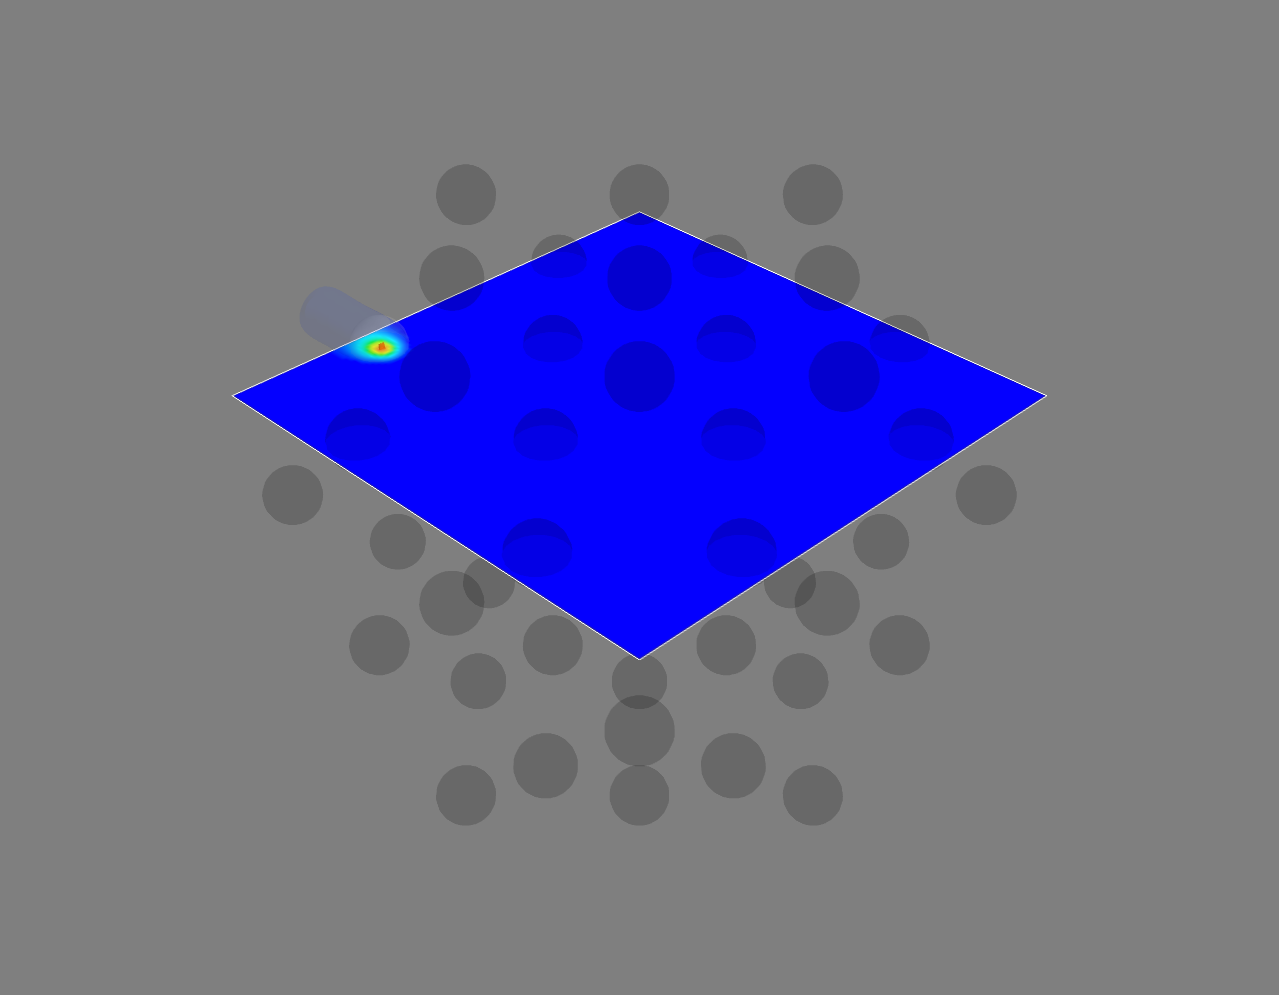
\includegraphics[width=.8\textwidth]{snapshot}\label{subfig: biasing_map}} \\
    \subfloat[]{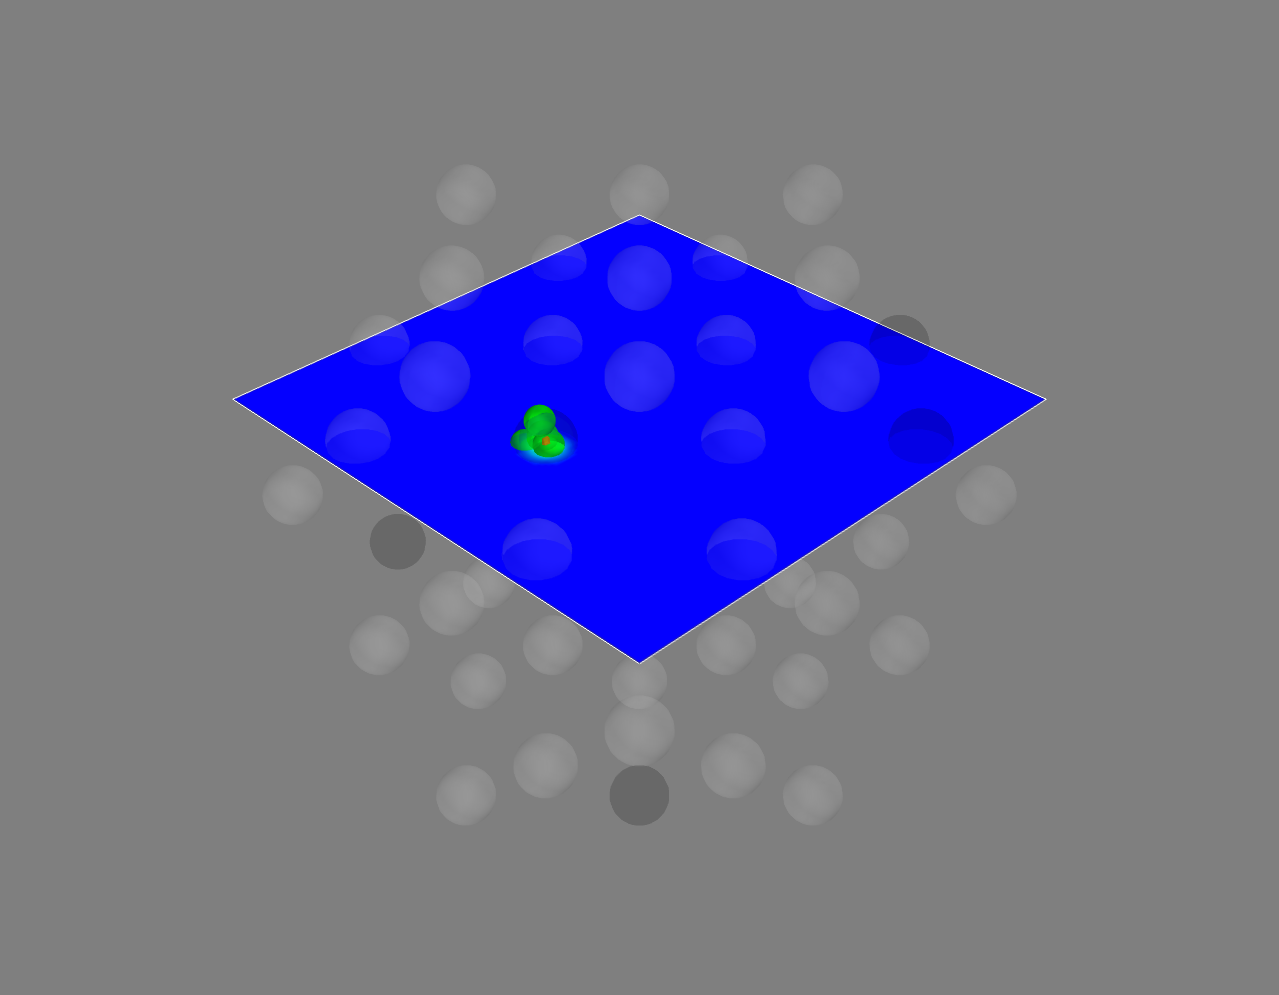
\includegraphics[width=.8\textwidth]{gc_positioning_snapshot}\label{subfig: insertian_trials}}
	\caption[Addition biasing with a Lennard Jones potential.]{These figures show slices of the three dimensional addition potential energy surface. a) shows the addition probability, with the red area most probable. b) shows the results of trial insertions, where the green spheres denote where insertions were attempted.}
	\label{fig:biasing}
\end{figure}
Figure \ref{subfig: biasing_map} shows an example map for atomic addition in a Au54 atom system, with an Au55 atom target.
Figure \ref{subfig: insertian_trials} shows the results of a few GCMC insertions with biasing, showing the focusing of the simulation on the missing atom.
The high density of insertions around the missing atom would not have been possible without the biasing.


\section{Conclusions}
In this chapter we have presented the development of both PES and the statistical mechanical ensembles used to search them.
We expanded the classical concept of a PES to a more generall mapping from positional variable space to energy space.
This expantion allowed for the implementation of experimentally derived PES, where the disagreement between experimental and computed results can be included in the PES.
Common experimental PESs were discussed, and their forces derived.
The implementation of various statistical mechanical ensembles, used for searching the PES for minima, was also discussed with a special focus on No-U-Turn-Sampling Hamiltonian Monte Carlo.
Grand Canonical Monte Carlo was also discussed, with an emphasis on the us of biasing to increase the overall acceptance rate.
Future work in this area may include the development of PESs which leverage 2 dimensional data, like STEM images, or ensembles which help to eliminate tuned parameters like parallel tempering.


\graphicspath{{./pdf/figures/}}
\tikzstyle{startstop} = [rectangle, rounded corners, minimum width=3cm, minimum height=1cm,text centered, draw=black, fill=red!30]
\tikzstyle{io} = [trapezium, trapezium left angle=70, trapezium right angle=110, minimum width=3cm, minimum height=1cm, text centered, draw=black, fill=blue!30]
\tikzstyle{process} = [rectangle, minimum width=3cm, minimum height=1cm, text centered, draw=black, fill=orange!30]
\tikzstyle{decision} = [diamond, minimum width=3cm, minimum height=1cm, text centered, draw=black, fill=green!30]
\usetikzlibrary{shapes.geometric}
\tikzstyle{database} = [cylinder, minimum width=3cm, minimum height=1cm, text centered, draw=black, fill=yellow!30, shape border rotate=90, aspect=0.25]

\chapter{Atomic Pair Distribution Function: \\Theory and Computation} \label{ch:pdf}
\section{Theory}
To properly understand the PDF and its limitations we need to derive its mathematics.
The PDF has been previously derived many times so it is not re-derived here.
This discussion of the PDF and its gradients use the notation of Farrow and Billinge. \cite{Farrow2009}
\subsection{Derivation}
\section{Theory}
To properly understand the PDF and its limitations we need to derive its mathematics.
The PDF has been previously derived many times so it is not re-derived here.
This discussion of the PDF and its gradients use the notation of Farrow and Billinge. \cite{Farrow2009}
\subsection{Derivation}
Many of the above techniques require the gradient of the PES.
This in turn requires the gradient of the PDF to be derived.
Mathematically treating thermal vibrations will also be discussed in this section.
Systems which are truly extended materials, like powders with particle sizes larger than 10nm, are best formulated as systems with periodic boundaries.
Thus, the equations for a periodically bound PDF need to be developed as well, with their gradients.
\subsection{Analytically Gradients}
Many optimization algorithms and simulations methodologies, including HMC, require not only the potential energy of a given configuration but also the forces acting on that configuration.
These forces are described by the gradient of potential energy of the system which in turn requires the gradient of the PDF.
As previously shown the PDF is the Fourier Transform of the Debye equation.
Since the Fourier Transform is expressed as an integral we can exchange the order of the gradient and the integral, allowing us to calculate the analytical gradient of the Debye equation and FFT the resulting function.
The Debye equation, with a Debye-Waller vibrational correction is
\begin{equation}
F(Q) = \frac{1}{N \langle f \rangle^{2}} \sum_{j\neq i} f_i^{*}(Q)f_j(Q) \exp(-\frac{1}{2}\sigma_{ij}^{2}Q^{2}) \frac{\sin(Qr_{ij})}{r_{ij}}
\end{equation}
where
\begin{eqnarray}
  \sigma_{ij}^{2} = (\vec{u}_{ij} * \hat{d}_{ij})^{2}\\
  \vec{u}_{ij} = \vec{u}_{i} - \vec{u}_{j}\\
  \hat{d}_{ij} = \frac{\vec{d}_{ij}}{r_{ij}}\\
  r_{ij} = ||\vec{d}_{ij}|| \\
  \vec{d}_{ij} =
  \begin{bmatrix}
    q_{ix} - q_{jx}\\
    q_{iy} - q_{jy} \\
    q_{iz} - q_{jz}
  \end{bmatrix}
\end{eqnarray}
where $Q$ is the scatter vector, $f_i$ is atomic scattering factor of the $i$th atom, and $r_{ij}$ is the distance between atoms $i$ and $j$ and has $q$ dependence. \cite{Jeong2002}
For simplicity's sake we will break up $F(Q)$ so that
\begin{equation}
F(Q) = \alpha \sum_{j\neq i} \beta_{ij} \uptau_{ij} \Omega_{ij} \label{eq:abto}
\end{equation}
where
\begin{eqnarray}
  \alpha = \frac{1}{N \langle f \rangle^{2}} \label{eq:alpha} \\
  \beta_{ij} = f_i^{*}(Q)f_j(Q)\label{eq:beta}\\
  \uptau_{ij} = \exp(-\frac{1}{2}\sigma_{ij}^{2}Q^{2}) \label{eq:tau}\\
  \Omega_{ij} = \frac{\sin(Qr_{ij})}{r_{ij}} \label{eq:omega}
\end{eqnarray}

\noindent The derivatives are as follows:
\begin{equation}
\frac{\partial}{\partial q_{i,w}} F{ (Q )} = \alpha \sum_{j} \beta_{ij} (\frac{\partial \uptau_{ij}}{\partial q_{i,w}}  \Omega_{ij} + \uptau_{ij} \frac{\partial \Omega_{ij}}{\partial q_{i,w}}) \label{eq:grad_fq}
\end{equation}
where
\begin{eqnarray}
  \frac{\partial \Omega_{ij}}{\partial q_{i,w}}  = \frac{Q\cos(Qr_{ij}) - \Omega_{ij}}{r_{ij}^{2}} (q_{i,w}-q_{j,w})\\
  \frac{\partial \uptau_{ij}}{\partial q_{i,w}} = \frac{\sigma_{ij}Q^{2} \uptau_{ij}}{r_{ij}^{3}}   ((q_{i,w} - q_{j,w}) \sigma_{ij}- ( u_{i,w} - u_{j,w})r_{ij}^{2})
\end{eqnarray}

Since $\vec{u}_{ij}$ is a variable as well, we need the derivative with respect to it as well.
Thus
\begin{eqnarray}
\frac{\partial}{\partial u_{i,w}} F{ (Q )} = \alpha \sum_{j} \beta_{ij} \frac{\partial \uptau_{ij}}{\partial u_{i,w}}  \Omega_{ij}\\
\frac{\partial \uptau_{ij}}{\partial u_{i,w}} = - \frac{\sigma_{ij}Q^{2} \uptau_{ij}}{r_{ij}}  (q_{i,w} - q_{j,w})
\end{eqnarray}
\subsubsection{Without ADPs}
Without ADPs the equations simplify down to
\begin{equation}
F(Q) = \frac{1}{N \langle f \rangle^{2}} \sum_{j\neq} f_i^{*}(Q)f_j(Q) \frac{\sin(Qr_{ij})}{r_{ij}}
\end{equation}
and
 \begin{equation}
\frac{\partial}{\partial q_{i,w}} F{ (Q )} = \alpha \sum_{j} \beta_{ij} \frac{\partial \Omega_{ij}}{\partial q_{i,w}}
\end{equation}
use of these equations, when ADPs are not appropriate (like at cryogenic temperatures), greatly speeds up the computation.

\subsubsection{Periodic Boundary Conditions}
Periodic boundary conditions can be helpful when simulating extended solids or large nanoparticles. In this case all the non-crystallinity is contained within the simulation box and the box is repeated to create the longer distance peaks observed in the PDF. To perform this we can break up the Debye equation into two main parts, the part that describes the interatomic distances within the simulation box and those between boxes. Neglecting the thermal motion portion:
\begin{equation}
  F(Q) = \frac{1}{N \langle f \rangle^{2}}(\sum_{j\neq i} f_i^{*}(Q)f_j(Q) \frac{\sin(Qr_{ij})}{r_{ij}} + \sum_{i,j} f_i^{*}(Q)f_j(Q) \frac{\sin(QR_{ij})}{R_{ij}})
\end{equation}
where
\begin{eqnarray}
  R = |\vec{r} + \vec{\nu}|\\
  \vec{\nu} = \gamma_1*\vec{a} + \gamma_2*\vec{b} + \gamma_3*\vec{c}
\end{eqnarray}
where $\gamma_{i}$ is the number of copies of the simulation box in the $i$th direction, and $\vec{a}, \vec{b}, \vec{c}$ are the lattice or superlattice directions.

%\input{pdf/pbc_adp}



\section{Computation} \label{sec:comp}
Simply deriving the equations for the PDF is not enough.
The many body nature of the PDF equation make analytical solution of the structure from the PDF impossible.
Thus, the PDF must be computed from a structural candidates and compared against experimental results to evaluate the reliability of the model.

\subsection{HPC and GPUs}
To properly solve the structure of materials the PDF will need to be computed many times and checked against experimental results.
This requires computation of the PDF, potentially over many atoms.
Calculating these PDFs requires a fast, highly parallized, computational framework.
\subsubsection{GPUs and Parallelization}
\begin{figure}
    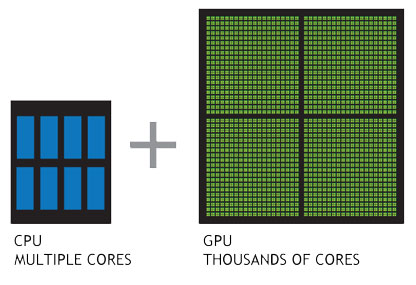
\includegraphics[width=\textwidth]{cpu-and-gpu}
    \caption{Comparison of the CPU and GPU chip architectures}
    \label{fig:cpu_vs_gpu}
\end{figure}
Computing the PDF is an embarrassingly parallel problem.
The basic procedure is to calculate the reduced structure factor $F(Q)$ for each atom pair and momentum transfer vector, sum over all the atom pairs, and Fourier transform the structure to the PDF.
The first part of this procedure is perfectly parallizable, as each atom pair is seperate from the others.
The summation over all the atomic reduced structure factors can be parallelized via distributed summing.
Lastly the FFT can be parallelized using existing parellel FFT algorithms.

GPUs are particularly well suted to the task of computing PDFs.
GPU chip architecture is designed to perform many task simultaniously by having potentially thousands of cores.

\subsubsection{Map from ij space to k space}
The above equations, although formally correct, are very ineffiecent. $F(Q)$ and its gradient are indexed over all the atoms twice, however there are symmetries that allow us to only compute over the atom pairs esentially mapping from an $n$x$n$ space, $ij$ space, to a $\frac{n(n-1)}{2}$ space, $k$ space.
For $F(Q)$ we apply the following mapping
\begin{figure}[!ht]
\begin{center}
\begin{tikzpicture}
    \node (E) at (0,0) {$E$};
    \node[right=of E] (F) {$E'$};
    \node[right=of F] (Z) {$Z$};
    \node[below=of F] (N) {$B'$};
    \node[below=of E] (M) {$B$};
    \draw[->] (E)--(F) node [midway,above] {$\psi$};
    \draw[->] (F)--(Z) node [midway,above] {$\Sigma$};
    \draw[->] (M)--(N) node [midway,below] {$\psi'$};
    \draw[->] (E)--(M) node [midway,left] {$\phi$};
    \draw[->] (N)--(Z) node [midway,left] {$\Sigma'$};
\end{tikzpicture}
\end{center}
\end{figure}
where $E$ denotes the atomic coordinates in $ij$ space, $E'$ denotes $F(Q)$ before the summation in $ij$ space, $B$ denotes the atomic pairs in $k$ space, $B'$ denotes $F(Q)$ in $k$ space, and $Z$ denotes the final summed $F(Q)$.  For the operators, $\phi$ denotes the mapping from $ij$ space to $k$ space $k = j + i * \frac{i - 1}{2}$, $\psi$ and $\psi'$ denote the $F(Q)$ operation in $ij$ and $k$ space, respectivly. $\Sigma$ denotes the sum over all the atoms.  

To properly define $\Sigma'$ we must establish whether $F(Q)$ is an even function.  
We can accomplish this by examining each of the portions of $F(Q)$, $\alpha, \beta ,\uptau, \Omega$.
$\Omega$ is even, since $r_{ij}$ is the interatomic distance, which is the same despite a flip of indicies, $Q$ does not depend on the atomic indicies, and since $Qr_{ij}$ is even so is $\sin{Qr_{ij}}$.  Thus, $\Omega$ is even.  Providing similar analysis to $\uptau$ we can see that while $\vec{u}_{ij}$ is odd, so is the unit displacement vector between the two atoms, thus the two odds cancel out.
Intuitivly this makes sense, since the $F(Q)$ equation is fundamentally interested in the interatomic distances which is even.  Thus, switching atom indicies does not change $F(Q)$.
Due to the even nature of the $F(Q)$ operator the $\Sigma'$ operator sums over all the atom pairs, and multiplies by two to reflect the double counting of the $\Sigma$ operator.

For the gradient a similar mapping is used:
\begin{figure}[h!]
\begin{center}
  \begin{tikzpicture}
    \node (E) at (0,0) {$E$};
    \node[right=of E] (F) {$E'$};
    \node[right=of F] (Z) {$Z$};
    \node[below=of F] (N) {$B'$};
    \node[below=of E] (M) {$B$};
    \draw[->] (E)--(F) node [midway,above] {$\psi$};
    \draw[->] (F)--(Z) node [midway,above] {$\Sigma$};
    \draw[->] (M)--(N) node [midway,below] {$\psi'$};
    \draw[->] (E)--(M) node [midway,left] {$\phi$};
    \draw[->] (N)--(Z) node [midway,left] {$\tilde{\phi}\Sigma$};
\end{tikzpicture}
\end{center}
\end{figure}

In this mapping, however, we use the $\tilde{\phi}\Sigma$ operator.  This operator simultaniously performs a reverse mapping from $k$ to $ij$ space, and a summation with the correct symmetry.  In this case the $\psi$ and $\psi'$ operators, which denote the $\grad{F(Q)}$ operator in $ij$ and $k$ space, are antisymmetric.  Intuitivly this makes sense as an extension of Newton's Second Law, since each particle's interation is felt oppositely by its partner.
\subsubsection{GPU Memory Allocation}
While GPUs are very fast computational engines they tend to be memory bound.
While a gradient array for a 10nm Au nanoparticle, consisting of 31,000 atoms and half a billion unique distances, occupies 1.5 TB of memory a single GPU's RAM allotment varies from 4GB on a NVIDIA GTX970 to 24 GB on a NVIDIA Tesla K80.
Thus, it is important to determine exactly how many atoms can fit on a GPU of arbitrary size as a funciton of the number of atoms and the $Q$ range.
The memory required per array is:
\begin{eqnarray}
    q [=] 3n\\
    d [=] 3k\\
    r [=] k\\
    scatter [=] nQ\\
    normalization [=] kQ\\
    omega [=] kQ\\
    F_{k}(Q) [=] kQ\\
    Sum [=] kQ\\
    Sum2 [=] kQ\\
    F(Q) [=] Q
\end{eqnarray}
where $n$ is the number of atoms, $k$ is the number of uniqe distances, $Q$ is the scatter vector.
Each of the above arrays are used in the computation and thus must be able to be held in memory.
Thus the number of atom pairs that can fit on a GPU with $am$ bytes of available memory is:
\begin{equation}
    k_{per GPU} = \frac{1}{16 Q + 16} \left(- 4 Q n - 4 Q + am - 12 n\right)
\end{equation}
If ADPs ar eincluded in the calculation, then the following arrays are also added to the memory allocaiton:
\begin{eqnarray}
    adps = 3n\\
    sigma = k\\
    tau = kQ
\end{eqnarray}
Thus the pair allotment is:
\begin{equation}
    k_{per GPU} = \frac{- 4 Q n - 4 Q + am - 24 n}{20 Q + 20}
\end{equation}

For the Gradient we need to calculate $F(Q)$ and its gradient, so the total memeory overhead is equal to the previously mentioned arrays plus:
\begin{eqnarray}
    g_omega = 3kQ \\
    g_fq = 3kQ \\
    rtn = 3nQ
\end{eqnarray}
Thus the gradient allotment is:
\begin{equation}
    \grad{k_{per GPU}} = \frac{- 16 Q n + am - 12 n}{32 Q + 16}
\end{equation}
For the gradient with ADPs the ADP gradient array is:
\begin{equation}
    g_tau = 3kQ
\end{equation}
Thus the allocation is:
\begin{equation}
    \grad{k_{per GPU}} = \frac{ - 16 Q n + am - 24 n}{48 Q + 20}
\end{equation}
These equations were solved by sympy as their validity is very important to the overal relyability of the software.
If the GPU is overallocated then the system may crash or return meaningless results.

\todo[inline]{Include Speed Benchmarks Here}

\graphicspath{{./bmk/figures/}}
\chapter{Benchmarking} \label{ch:bmk}
\todo[inline]{This entire section needs some rewritting to distinguish this from the paper}
\todo[inline]{Also some introduction would be great}
\todo[inline]{this just needs a lot of work}
\section{Introduction}
The NUTS-HMC system was tested on a series of nanoparticle (NP) benchmarks.
The purpose of these benchmarks is to test the ability of the NUTS-HMC system to reproduce the target PDF and its associated structure.
Systems were chosen for their size, crystallinity, and interfacial differences.

\section{PDF}
The formation of NPs with both crystallographic and non-crystallographic structures \cite{Marks1994} and with different chemical patterns \cite{Ferrando2008} are well documented.
For simplicity, we chose monometallic Au clusters as benchmarks and considered two groups of structures with different size and degrees of structural disorder in order to assess the reliability and efficiency of our HMC method for solving atomic structures from PDFs.
The first group consists of \ce{Au55} clusters with different degrees of disorder, including a crystalline cluster structure in $O_h$ (Octahedral) symmetry, a structure with a disordered surface, and an amorphous structure.
The second group consists of the crystallographically solved \ce{Au102} structure as in the \ce{Au102MBA44} nanocrystals \cite{Jadzinsky2007,Li2008}.
We used optimized structures from the Density Functional Theory (DFT) as target structures and generated the corresponding PDF, $G_{_\mathrm{obs}}$, according to
\begin{equation}
\label{Eq:Gdef}
  G_{_\mathrm{obs}} = \frac{2}{\pi} \int_{Q_\mathrm{min}}^{Q_\mathrm{max}} Q[S_{_\mathrm{obs}}(Q) - 1] \sin{\left (Q r \right )}\, dQ
\end{equation}
where $S_{_\mathrm{obs}}$ is the target structure's structure factor.
Since all the target structures were optimized by DFT at zero Kelvin the target and model PDF profiles were calculated at zero temperature, with no atomic displacement parameters (ADPs).
However, ADPs would have a considerable impact on the calculation of the PDF, especially for nanoparticles at non-zero temperatures.


Spin-polarized  DFT calculations were carried out using the Vienna ab initio simulation package (VASP) \cite{Kresse1993, Kresse1994} within the  Perdew-Burke-Ernzerhof (PBE) exchange-correlation functional \cite{PERD1996}.
The projected augmented wave method \cite{Blochl1994} and a kinetic energy cutoff of 400 eV were used.
Structural optimization was performed until the total energy and ionic forces were converged to 10$^{-6}$ eV and 10 meV/\AA, respectively.
The  amorphous \ce{Au55} structures were generated by simulated annealing using the classical embedded atom method potential \cite{Sheng2011}.
Different annealing temperatures between 1200 K and 1670 K (bulk melting temperature of Au) were used and the thermally equilibrated structures were cooled down to 300 K before minimization at 0 K.
Further optimization using DFT leads to total energies that vary within 1-2 eV among different amorphous structures  and the lowest energy one was used as the target structure. The target structure of \ce{Au102} was taken as the \ce{Au102} core of the DFT-optimized \ce{Au102MBA44} cluster \cite{Li2008}.

All systems were refined using a PES  which consists of a linear combination of $Rw$, the repulsive and attractive thresholded spring potentials.  The total potential energy in the Hamiltonian in Eq. (\ref{Hamiltonian}) is expressed as:
\begin{eqnarray}\label{eq:Ucomp}
  U(q) = U_{Rw}(q) + U_\mathrm{spring}(q, R_\mathrm{min}) + U_\mathrm{spring}(q, R_\mathrm{max})
\end{eqnarray}
The thresholded spring potentials are based on those previously proposed on by Peterson \cite{Peterson2014}, i.e.  $U_\mathrm{spring}(q, r_{t}) = \frac{\kappa}{2}\sum_{i, j}(r_{i, j}-r_t)^{2}$  for all atomic distance $r_{i,j}$  outside the bounds of the spring threshold $r_t$.
The resulting restoring forces on the out-of-bound atoms  bring the system back within the bounds of the PDF, $R_\mathrm{min}$ and $R_\mathrm{max}$, and therefore preventing the system from exploding or collapsing.
Otherwise,  incorrect refinements may result by having atomic pair distances out of the PDF bounds.  $\kappa$ is the spring constant in eV/\AA~and the $Rw$ potential is converted from unitless to eV via multiplication by a conversion factor $\lambda$.

Whereas the choice of the absolute values of $\lambda$ and $\kappa$ is somewhat arbitrary, their relative values are important in determining which  term in Eq.~(\ref{eq:Ucomp}) dominates the PES, especially when considering the effect of the simulation temperature.
Generally, the ratio between the total potential energy and the temperature determines how much random motion will dominate the dynamics; a lower ratio implies that random motion will play a large role in the dynamics.
The ratio between $\lambda$ and $\kappa$ of each spring describes how far the PDF can push the system below or above the bounds set by the spring potentials.
Heuristically, too stiff a spring  forbids the system to access new configurations, e.g.  high energy ``transition states'' which may involve shorter bonds or a larger system size.
Conversely, too small a spring constant makes it slower for the system to snap back within bounds and may lead to an explosion or implosion of the system, leaving the dynamics to drift aimlessly.

\subsection{Model Parameters}
Unless otherwise stated, the PDFs of the target and starting structures were generated using Eqn. (\ref{Eq:Gdef}) with a step of $\delta R=.01$~\AA, $Q_\mathrm{min}=0.1$~\AA$^{-1}$,  $Q_\mathrm{max}=25.0$~\AA$^{-1}$.
$R_\mathrm{min}$ and $R_\mathrm{max}$ correspond to the first minimum before the first PDF peak and that after the last PDF peak, respectively, which ensure that the full meaningful region of the PDF is modeled.  For each of the simulations, the Q resolution was calculated by
\begin{equation}
\delta Q=\frac{\pi} {R_\mathrm{max} + \frac{12 \pi}{Q_\mathrm{max}}}
\end{equation}

The HMC simulation was run with $N=300$  iterations, a target acceptance rate of 0.65, and an average starting momentum for each NUTS iteration  of 10 eVfs/\AA. Both  repulsive and attractive spring potentials are used with $\kappa=200$ eV/\AA ~and thresholds matching $R_\mathrm{max}$ and $R_\mathrm{min}$ of the PDF, respectively.  $\lambda=$ 300 eV was used as conversion factor for $Rw$. Each simulation was run with a pair of Nvidia GTX970 graphics cards, with one card partially occupied with desktop visualization.


\foreach \n in {au55sr, au55sd, au55a, au102tp, au147}{
    \input{bmk/\n}
}

\section{PDF with ADPs}
\foreach \n in {adp_50
%, adp_random, adp_janus
}{
    \input{bmk/\n}
}
\begin{enumerate}
\item Basic 50\% larger magnitude
\item Random addition to APDs
\item Janus ADPs
\end{enumerate}

\graphicspath{{dp/figures/}}
\chapter{X-ray Total Scattering Data Acquisition and Processing} \label{ch:dp}
\section{Introduction}
X-ray total scattering experiments are generally performed at synchrotron light sources, as only these sources can provide the needed flux, energy, and high momentum transfer vectors needed to obtain reliable PDFs. \cite{Chupas2003, Dykhne2011}
Despite the need for a dedicated facility to perform the total scattering experiments, the experiments themselves are fairly forgiving, allowing for reactive gasious environments, experiment temperatures ranging from 2 \si{K} to 1200 \si{K}, and even electrochemical cycling. \cite{Chupas2008, Petkov2013, Redmond2012}
The rapid PDF data aquesition associated with 2D area detectors creates a data management problem, as 96 hours of beamtime could result in almost $10,000$ images which need to be associated with the experimental conditions and detector metadata. \cite{Chupas2003}
 Finaly, all this data needs to be processed by masking bad pixels and regions, integrating azimuthally, and converting the scattering data to the PDF. \cite{Kieffer2013, Juhas2013, Yang2014, Pauw2014, Billinge2012}

%\section{Data Storage and Management}

Processing the raw pixel intensities to the PDF is very important as we are extracting most of our interesting information out of very high $Q$ data.
This data relies on good statistics and sound background subtraction.
Talk about papers from Billinge Group with thin film PDF and dilute NP solutions.
Diagram of the overall data processing workflow.
Discuss the NSLS-II data stack.
\begin{figure}
\centering
\begin{tikzpicture}[thick,scale=0.6, every node/.style={scale=0.6}]
    \node (img) [startstop] at (0,0) {Image Data};
    \node [database, right=of img] (fs)  {FileStore};
    \node[startstop, below=of img] (imeta) {Image Metadata};
    \node[startstop, below=of imeta] (emeta) {Environmental Metadata};
    \node[startstop, below=of emeta] (bmeta) {Beamline Metadata};
    \node[startstop, below=of bmeta] (smeta) {Sample Metadata};
    \node[database, right=of emeta] (mds) {MetadataStore};
    \node[process, right=of mds] (db) {DataBroker};
%     \node[io, right=of db] (lfg) {Load Data};
%     \node[io, below=of lfg] (lbg) {Load Background};
%     \node[process, right=of lfg] (maskfg) {Mask Data};
%     \node[process, right=of lbg] (maskbg) {Mask Background};
%     \node[process, right=of maskfg] (ifg) {Azimuthally Integrate Data};
%     \node[process, right=of maskbg] (ibg) {Azimuthally Integrate Background};
%     \node[process, right=of ifg] (bgsubs) {Subtract Background};

%     \draw[->] (img) -- ++(0,1) -- ++($(fs)+(0,1)$)node[] -- (fs);
%     \draw[->] (F)--(Z) node [midway,above] {$\Sigma$};
%     \draw[->] (M)--(N) node [midway,below] {$\psi'$};
%     \draw[->] (E)--(M) node [midway,left] {$\phi$};
%     \draw[->] (N)--(Z) node [midway,left] {$\tilde{\phi}\Sigma$};
\end{tikzpicture}
\caption{Database Loading Workflow. Data is loaded from various sources, including images and text files, into the FileStore and MetadataStore databases. Data is then retrieved from the databases using the databroker.}
\end{figure}
\subsection{MetadataStore Side Loading}
Design of sidewinder-spec for loading the data into metadatastore.
Most of the design considerations went into the loaders, which are different for each experiment.

\subsection{Detector $Q$ resolution} \label{subsec:qres}
To properly azimuthaly integrate the images taken from the detector the $Q$ resolution of the pixels must be calculated.
Integrating using even bins will cause pixels which are not on the same ring to be binned together, causing the incorrect value of $I(Q)$ to be obtained and a larger standard deviation in the integrated data.
To properly calculate the $Q$ resolution the resolution of each of the pixels in $2\theta$ must be calculated.
\begin{figure}
    \centering
    \begin{tikzpicture}
        \draw (0,0) node[anchor=north]{$A$}
          -- (4,0) node[anchor=north]{$C$}
          -- (4,4) node[anchor=east]{$B$}
          -- cycle;
        \draw (0,0) node[anchor=north]{$A$}
          -- (4,0) node[anchor=north]{$C$}
          -- (4,6) node[anchor=south]{$B'$}
          -- cycle;
    \end{tikzpicture}
    \caption{Scattering onto a flat detector}
    \label{fig:scattering_digram}
\end{figure}
Figure \ref{fig:scattering_digram} shows the scattering of x-rays onto a flat image plate detector.
In this diagram the bottom of the $n$th pixel is $B$ while the top is $B'$.
The resolution of this pixel in $2\theta$ is $\angle BAC - \angle B'AC$.
Thus the resolution, calculated from the distances is
\begin{equation}
\Delta 2 \theta = \arctan{\frac{b}{d}} - \arctan{\frac{t}{d}}
\end{equation}
where d is the sample to detector distance, b is the distance to the bottom of a pixel, and t is the distance to the top of that pixel.
Note that these distances need to have been corrected for detector tilt and rotation.
Thus the resolution of a pixel in $Q$ is
\begin{equation}
\Delta Q = \frac{4\pi(\sin{\arctan{\frac{b}{d}}} - \sin{\arctan{\frac{t}{d}}})}{\lambda}
\end{equation}
where $\lambda$ is the x-ray wavelength.

For a Perkin Elmer image plate, like the one used at the NSLS-II's XPD and the APS's 11-ID-B, the resolution function is shown in \ref{fig:res_func}.
For the same detector the number of pixels per $Q$ is shown in \ref{fig:pixel_hist}
\begin{figure}[!ht]
  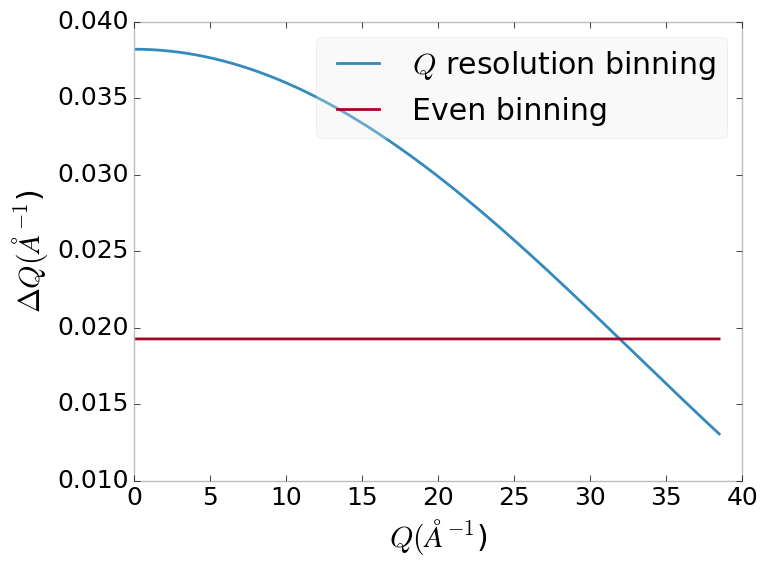
\includegraphics[width=\textwidth]{res}
\caption{$Q$ resolution as a function of $Q$.}
\label{fig:res_func}
\end{figure}

\begin{figure}[!ht]
  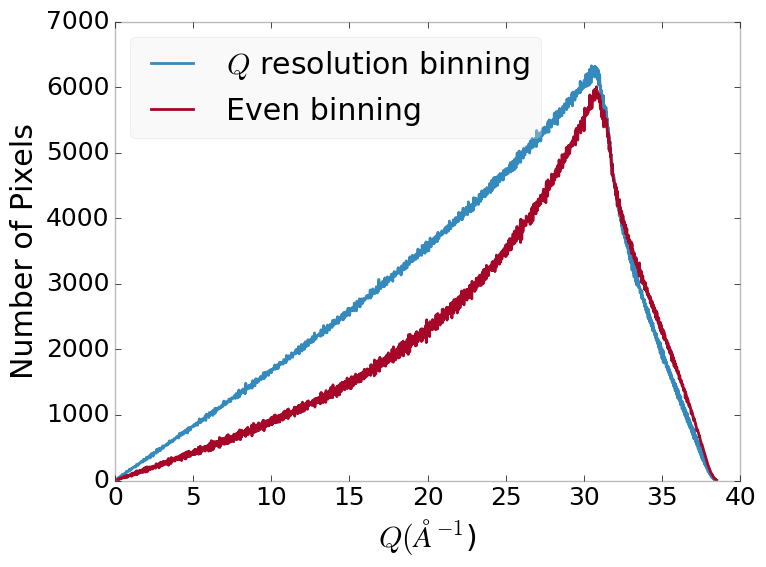
\includegraphics[width=\textwidth]{pixels}
\caption{Number of pixels as a function of $Q$, binned at the $Q$ resolution of the detector.}
\label{fig:pixel_hist}
\end{figure}

\section{Automated Mask Generation} \label{subsec:mask}
\subsection{Introduction}
Detector masking is an important part of any x-ray scattering workflow as dead/hot pixels, streak errors, and beamstop associated features can be averaged into the data changing the signal and its statistical significance.
While some features, like the beamstop holder, can be easily observed and masked by hand other are much more difficult to observe even on large computer monitors.
Additionally, while dead/hot pixels and streaks are usually static the hot pixels associated with textured or single crystal scattering or cosmic rays are not.
Thus, coming up with an automated method for finding such erroneous pixels is important, especially as high flux diffraction beamlines can generate data very quickly.

While this problem can be quite complex in the most general case, we can use the annular symmetry of the powder scattering pattern to our advantage, by comparing a pixel against pixels in the same ring.
Since non-textured powder scattering should produce the same pixel intensity for a given ring we can mask any pixels which are $\alpha$ standard deviations away from the mean.
This method relies on the aforementioned pixel binning algorithm, as using miss sized bins will cause some pixels which should be in separate rings to be put together, and others which should be in the same ring to be separated.
In that case the masking algorithm will overestimate the number of pixels to be masked due to the additional statistical variation in the sample.

\subsubsection{Algorithm Design}
The masking algorithm procedure takes in the image and a description of the pixel positions in either distance from the point of incidence or in $Q$.
The image is then integrated twice, producing both the mean $I(Q)$ and the standard deviation of each $I(Q)$ ring.
The mask is created by comparing the pixel values against each ring's standard deviation and threshold $\alpha$.
Note that the threshold can be a function of distance from the point of incidence or $Q$.

\subsubsection{Test Cases}
To study the effectiveness of the masking we ran the algorithm against both simulated experimental data.
In the case of the simulated data four systems were created:
1) dead/hot pixels with varying numbers of defective pixels,
2) beamstop holder with varying beamstop holder transmittance,
3) rotated beamstop holder with varying beamstop holder transmittance,
and 4) beamstop holder with dead/hot pixels.
The base scattering was produced by
\begin{equation}
I = 100\cos(50r)^{2} + 150
\end{equation}
where $r$ is a pixel's distance from the beam point of incidence.
The positions of the dead/hot pixels were chosen at random as was the dead or hot nature of the defect. Dead pixels had values from 0 to 10, while hot pixels had values from 200 to 255.
The beamstop was positioned at the vertical center of the detector with an initial width of 60 pixels and final width of 120 pixels.
The height of the beamstop was 1024 pixels.
The beamstop was calculated to attenuate the x-ray scattering signal at various transmittance, as various beamstop holder materials have different transmittance.
Two version of the masking algorithm were run for each test case, one using the standard even bin sizes for the integration step, and one where the bin sizes are tuned to the pixel $Q$ resolution as discussed in \ref{subsec:qres}.

\subsubsection{Results and Discussion}
\foreach \n in {100, 300, 500, 1000}{
\begin{figure}
  \centering
  \foreach \m in {masked}{
    \subfloat[]{\includegraphics[width=.5\textwidth]{bad_bin_dead_pixel_\m_\n}}
    \subfloat[]{\includegraphics[width=.5\textwidth]{dead_pixel_\m_\n}}
    }
\caption[Generated dead/hot pixel masks for a detector with $\n$ bad pixels.]{Generated dead/hot pixel masks for a detector with $\n$ bad pixels. a) the standard even bin mask and b) the $Q$ resolution binned mask. The bad pixels are noted with open circles, masked pixels are noted with closed circles.}
  \label{fig:dead_pixel_\n}
\end{figure}
}

\foreach \n in {10, 30, 50, 90}{
\begin{figure}
  \foreach \m in {raw, masked, missed}{
    \subfloat[]{\includegraphics[width=.3\textwidth]{\m_\n}}
    }
  \caption[Generated beamstop holder masks for a beamstop holder with $\n\%$ transmittance.]{Generated beamstop holder masks for a beamstop holder with $\n\%$ transmittance. a) the raw image, b) the masked image, c) and the missed pixels}
  \label{fig:bs_\n}
\end{figure}
}

\begin{figure}
        \foreach \m in {raw, masked, missed}{
        \subfloat[]{\includegraphics[width=.3\textwidth]{rotate_\m_50}
        }}
    \caption{Generated beamstop holder masks which is rotated away from vertical}
    \label{fig:rot_bs}
\end{figure}

Figures \ref{fig:dead_pixel_100}-\ref{fig:bs_90} show the results of the masking algorithm on simulated images.
The dead/hot pixel masking shows the importance of using the $Q$ resolution based bin sizes as the even bin based mask have a tendency to over mask the image, removing pixels which contain valuable signal.
This over-masking is caused by pixels being improperly associated with one another by the even bins.
Figure \ref{fig:dead_pixel_100} indicates that the masking algorithm, with the proper binning, masks the image perfectly, with no missed bad pixels or good pixels masked.
This is not the case in figures \ref{fig:dead_pixel_300} - \ref{fig:dead_pixel_1000} as we can see pixels which should have been masked but were not.
Despite these missed pixels no pixels were improperly masked in any of the well binned images.
These test cases are actually more difficult than experimental data, as the dynamic range of most detector causes the dead/hot pixels and single crystal/texture peaks to be orders of magnitude away from the desired signal.

The beamstop holder masks shown in figures \ref{fig:bs_10} - \ref{fig:bs_90}, which were all run with the $Q$ resolution binning show similar results across the transmittance range, missing only a small part of the beamstop holder near the point of incidence.
Near this point the beamstop holder becomes a statistically significant part of the total number of pixels in a given ring, thus it can not be masked out using a statistical search of the rings.
For most PDF and XRD studies this small area can be masked automatically by masking all the pixels who's distance from the point of incidence is smaller than a given radius $r$, or can be neglected outright as the area is not used in the analysis or refinement.
Similar results were produced for beamstop holders which were rotated away from the vertical position, as shown in figure \ref{fig:rot_bs}

\begin{figure}
    \foreach \m in {raw, masked}{
        \subfloat[]{\includegraphics[width=.5\textwidth]{exp_\m}}
    }
    \caption[Masked experimental data.]{Masked experimental data. a) the raw image, b) the mask}
    \label{fig:masked_exp}
\end{figure}

\begin{figure}
    \foreach \m in {raw, masked}{
        \subfloat[]{\includegraphics[width=.5\textwidth]{single_xtal_\m}}
    }
    \caption[Masked experimental data with Pt single crystal signal.]{Masked experimental data with Pt single crystal signal. a) the raw image, b) the mask}
    \label{fig:masked_single_xtal}
\end{figure}

\begin{figure}
    \foreach \m in {raw, masked}{
        \subfloat[]{\includegraphics[width=.5\textwidth]{combined_\m}}
    }
    \caption[Masked experimental data with Pt single crystal signal using figure's \ref{fig:masked_exp} mask as a starting mask.]{Masked experimental data with Pt single crystal signal using figure's \ref{fig:masked_exp} mask as a starting mask. a) the raw image, b) the mask}
    \label{fig:combined}
\end{figure}

Working with actual experimental data, obtained at the Advanced Photon Source beamline 11-ID-B, shows the difficulty of masking images which have low photon counts.
While the masking of experimental data taken with longer exposures, consisting of 250 .2 second shots, shown in figure \ref{fig:masked_exp} provides very sharp edges to the beamstop holder, and very little extra masking beyond the occasional dead pixel, this is not the case for the single crystal data.
The single crystal data is more problematic because of its short exposure time and low flux, with 500 frame at a .1 second exposure and having shrunk the beam size.
The low flux is to prevent the very strong single crystal peaks from damaging the detector.
However, this causes the image to be less statistically viable then ideal, causing problems with the mask as seen in figure \ref{fig:masked_single_xtal}.
This can be alleviated to some degree by using the previously generated mask as a starting mask for the single crystal image, as shown in \ref{fig:combined}.
While the masking algorithm still produces many diffuse masked pixels, they are far fewer, this may be due to the removal of the beamstop which could have contributed to the large standard deviation in figure \ref{fig:masked_single_xtal}.


\subsubsection{Conclusions}
In this section the masking algorithm, which relies on both $Q$ resolution based binning and a statistical approach to azimuthal symmetry, was developed.
The focus of this algorithm was to remove many unwanted detector features associated with pixel defect, beamstop holder associated scattering attenuation, and single crystal/texture peaks.
Simulated data was used to evaluate the beamstop holder and dead/hot pixel masking capacity, while experimental data was used to check for single crystal and texture based masking.
$Q$ resolution based binning was shown to be very important to avoid over-masking.
The ability of the mask writer to mask images is somewhat limited by the overall statistical image quality, although some deficiencies can be obtained by using previously generated masks as starting points.
This masking algorithm is now in use in the data processing workflow and will be available in scikit-beam soon.


\section{Automated Image Azimuthal Integration} \label{subsec:int}
Using the $Q$ resolution binning and masking developed in sections \ref{subsec:qres} and \ref{subsec:mask} the images can be properly integrated.
Generally, images are integrated by taking the mean value of the pixels in a ring.
However, other statistical measures of the average value can be used, like the median.

Figures \ref{fig:workflow_no_mask}-\ref{fig:workflow_auto_mask} show the importance of masking and the choice of average function.
All the figures were produced using the same dataset, 50 \si{\degree}C \ce{Pr2NiO4} taken at the APS's 11-ID-B on a Perkin Elmer area detector.
The automatic masking alpha was $3$ standard deviations from the mean.
While it is difficult to observe the changes the mask causes in the full $I(Q)$ plot (subfigures a) and b)), the standard deviation plots show the effect of bad pixels on the data (subfigure c)).
Subfigure c) for figures \ref{fig:workflow_no_mask}-\ref{fig:workflow_auto_mask} shows that removal of the beamstop holder lowers the low $Q$ standard deviation from around .1 to almost .01 out to 15 \iA.
The high $Q$ subfigures d) and f) in figures \ref{fig:workflow_no_mask}-\ref{fig:workflow_auto_mask} show the ``kink'' effect of the detector edge and beamstop holder, where there is a dip in the $I(Q)$ scattering when the rings include the edge of the detector.
This effect seems to be due to both errors in the edge pixel intensity and the beamstop holder as masking of the edges only seems to provide only partial removal of the issue.
It is important to note that while integration using the mean of the ring has issues with only the edge mask, as evidenced by the change in slope in \ref{fig:workflow_edge_mask} d) around 29.5 \iA, the median integration does not include this error.
Ideally the detector would have a normal distribution of pixel intensity for a given ring, which would imply an equivalency between the mean and median $I(Q)$ values.
Despite the closeness of the mean and median once the final mask has been created, it seems that the median is more reliable, as it was less effected by the beamstop holder in figure \ref{fig:workflow_edge_mask}.
Thus, for subsequent integrations discussed in this work the median is used to avoid any defective features that the masking algorithm may have missed.

%\begin{landscape}
\foreach \n/\o in {no_mask/with no mask, edge_mask/with only an edge mask, auto_mask/combining an edge mask and the automatically generated mask}{
    \begin{figure}[!h]
    \centering
    \foreach \m in {img, mask, ave, std, high_q_ave, high_q_std}{
        \subfloat[]{\includegraphics[width=.4\textwidth]{\n_\m}}
        }
    \caption[Masking, average, and standard deviation of an example x-ray total scattering measurement with \o.]{Masking, average, and standard deviation of an example x-ray total scattering measurement. This image was produced \o. a) the image, b) the mask, c) the mean and median values, d) the standard deviation (normalized to the median), e) a closeup of the 28 \iA to 31 \iA $Q$ range for the mean and median, f) 28 \iA to 31 \iA $Q$ range for the standard deviation}
    \label{fig:workflow_\n}
    \end{figure}
}
%\end{landscape}

\section{Conclusions}
This chapter developed and analyzed the proper data processing and reduction methodology for producing reliable $F(Q)$ data from x-ray total scattering measurements.
Binning at the $Q$ resolution of the detector was found to be key to the data processing.
The primary outcome of using the $Q$ resolution binning was an enhancement in effectiveness for the masking algorithm, producing much fewer false positives for dead pixels.
This masking approach was then applied to the integration of experimental data taken at the APD's 11-ID-B beamline.
The automaticly generated masks, when combined with edge masks, were found to greatly reduce the overall standard deviation of the pixel intensity and produce a smoother $F(Q)$ at high $Q$, enabling the use of much higher $Q$ data in the PDF.
Different statistical measures used in the azimuthal integration was also compared.
This comparison showed that the median was a more reliable statistic for integration with data which had more detector defects.
However, upon properly masking it was shown that these metrics were almost identical.
The masking induced similarity between the mean and median shows that the rings, when integrated, may form a Gaussian distribution.
The distribution of the pixel intensities for strongly and weakly scattering samples may be investigated in future work.

% \chapter{Annealing and Aggregation of 2nm \\\ce{Au} Nanoparticles}
\todo[inline]{If we are going to keep this we need to get a lot done in terms of modeling}
\section{Experiments}
\subsection{NP Synthesis}
\subsection{X-ray Total Scattering Measurements}
\section{Data Processing}
\section{Data Analysis}
\section{Simulation}
\section{Structural Analysis}
\section{Conclusions}

\graphicspath{{./pno/figures/}}
\chapter{Phase Changes and Annealing Dynamics of \ce{Pr2NiO4} and its derivatives} \label{ch:pno}
\section{Introduction}
\ce{Pr2NiO4} (PNO) electrodes provide higher power density than \ce{La_{0.8}Sr_{0.2}MnO3} (LSM), and is more stable than \ce{(La_{0.60}Sr_{0.40})_{0.95}(Co_{0.20}Fe_{.80})O_{3-x}} (LSCF), which is known to rapidly degrade in performance. \cite{Zhou2012}
PNO's high performance between 600-900 $^\circ$C is associated with its high activity towards the oxygen reduction reaction (ORR), which stems from PNO's high oxygen diffusion and surface exchange coefficients, substantial oxygen over-stoichiometry, and large oxygen ion conduction paths through the unit cell. \cite{Yashima2008}
Despite these advantages, PNO's tendency to partially decompose into PrOx and other phases is particularly challenging. \cite{Dogdibegovic2016}
Full cell operation after 500 hours at 750 $^\circ$C and 0.8 V shows major decomposition of the parent PNO phase, while the performance degrades by only 4\%.
Such significant changes in phase and relatively small changes in performance further assure the necessity for understanding the phase evolution in nickelate cathodes during operation.
To address these disparity in performance and phase degradation PDF and XRD analysis may be able to examine these issues from both long and short range ordering perspectives.

\section{Experiments}
\subsection{\ce{Pr2NiO4} Synthesis}
\ce{Pr2NiO4} was synthesized using the standard approach, as detailed in the work by Dogdibegovic et al. \cite{Dogdibegovic2016}
The nickelate powder was initially prepared via the glycine-nitrate process.
This was followed by thermal annealing at 1080 $^\circ$C for 10 hours in air.

\subsection{X-ray Measurements}
X-ray total scattering and x-ray powder diffraction experiments were performed at the APS's 11-ID-B beamline.
An x-ray energy of 86.7 keV, .145 \AA was provided by the beamline monochromator.
The detector was moved between a 20cm and a 95 cm sample to detector distance to measure the x-ray total scattering and x-ray diffraction patterns.
Various PNO samples were annealed on the beamline during x-ray measurement.
\section{Data Processing}
The data was calibrated at each of the detector positions using a \ce{CeO2} standard via pyFAI. \cite{Kieffer2013}
The images were corrected for a .95 x-ray polarization.
Masks were produced for both the foreground and background images.
The foreground masks were produced using both a 30 pixel edge mask and a 2.5$\sigma$ automatic mask as discussed in chapter \ref{ch:dp}.
The background masks were produced by using the foreground mask as a starting mask with a 2.5$\sigma$ automatic mask.

The foreground and background images were then integrated using the $Q$ resolution binning discussed in chapter \ref{ch:dp}.
The resulting $I(Q)$ data were corrected for their number of frames and $I_{00}$.
Finally the corrected background $I(Q)$ was subtracted from the foreground $I(Q)$.

Each PDF was generated with a
$Q_{min}$ of 1.5,
$Q_{max}$ of 29.,
$R_{poly}$ of .9,
$R_{max}$ of 40.
descriptions of these parameters can be found in the work by Juhas et. al. \cite{Juhas2013}

\section{Data Analysis}
\subsection{Intra Sample Comparison}
\subsubsection{PDF}
As figures \ref{fig:S1_0_to_40_pdf} and \ref{fig:S1_0_to_10_pdf} show the as synthesized PNO undergoes very little change in structure according to the PDF.
The PDF does show some broadening at around 3.5 and 8.5 \AA, but the peak shifts themselves are fairly limited.
This implies that the as synthesized PNO structure is stable at least for the 1 hour that the sample was held at 750 $^\circ$C.

\begin{landscape}
\foreach \n/\o in {S1/as synthesized PNO , S2/PNO annealed at 750 $^\circ$C for 25 hours }{
    \foreach \m/\p in {0_to_40/the full PDF, 0_to_10/a close up on the short range section}{
        \begin{figure}
            \includegraphics{\n/\m_gr}
            \caption{PDF as a function of temperature for \o showing \p}
            \label{fig:\n_\m_pdf}
        \end{figure}
    }
}
\end{landscape}


\subsubsection{$I(Q)$}
The annealed samples figures, \ref{fig:S2_0_to_40_pdf} and \ref{fig:S2_0_to_10_pdf}, tell a rather different story.
In this case the PDF shows significant peak shifts and broadening, especially at higher interatomic distances.
Some peaks completely disappear, like the peak at 12 \AA.
Similar results were also observed for samples with longer annealing times, as shown in the appendix.
\begin{landscape}
\foreach \n/\o in {S1/as synthesized PNO , S2/PNO annealed at 750 $^\circ$C for 25 hours }{
    \foreach \m/\p in {0_to_12/the full XRD, 0p8_to_5/a close up on the low $Q$ section}{
        \begin{figure}
            \includegraphics{\n/\m_chi}
            \caption{$I(Q)$ as a function of temperature for \o showing \p}
            \label{fig:\n_\m_iq}
        \end{figure}
    }
}
\end{landscape}

\subsection{Inter Sample Comparison}
Figures \ref{fig:s1-5_high-temp_chi} and \ref{fig:s1-5_full_high-temp_gr} show a very interesting contrast.
Figure \ref{fig:s1-5_high-temp_chi} show significant differences in the $I(Q)$ between the as-synthesized and annealed PNO, which could be associated with the more degradation present in the annealed samples.
However, figure \ref{fig:s1-5_full_high-temp_gr} shows very little difference in the PDF between the various annealing times.
This discrepancy seems to point to some kind of disorder which changes the interatomic distances very little but changes the symmetry enough to change the Bragg reflections.
\begin{landscape}
\foreach \n in {high-temp}{
    \foreach \m in {
%    short, medium, long
    full}{
        \begin{figure}
            \includegraphics{S1-5_\m_\n_gr}
        \caption[Comparison of PNO sample PDFs as a function of annealing time \n]{Comparison of PNO sample PDFs as a function of annealing time \n}
        \label{fig:s1-5_\m_\n_gr}
        \end{figure}
    }
    }
\end{landscape}

\begin{landscape}
\foreach \n in {high-temp}{
  \begin{figure}
    \includegraphics{S1-5_full_\n_chi}
    \caption[Comparison of PNO sample $I(Q)$ as a function of annealing time \n]{Comparison of PNO sample $I(Q)$ as a function of annealing time \n}
    \label{fig:s1-5_\n_chi}
  \end{figure}
}
\end{landscape}


\section{Simulation}
Simulations have not been run yet on these PNO samples.
Solving the structures of these samples is expected to be more difficult than the NP benchmarks previously solved.
The difficulty of these simulations is due to:
\begin{enumerate}
    \item The PDF's insensitivity to the oxygen positions, due to the poor x-ray scattering off the very electron poor oxygen.
    \item The large difference in mass between the oxygen and other atoms, causing the dynamics of the simulation to be governed by oxygen motion, necessitating long simulation times to obtain movement of the other atoms.
    \item The large parameter space caused by potential defects and degradation products.
    Without knowing that the starting phase is pure, it is difficult to even produce starting structures, since the simulation will need to explore all the potential defect/degenerated structures.
\end{enumerate}
%\subsection{Small Box}
%\subsection{Large Box}
%\section{Structural Analysis}
\section{Conclusions}
X-ray total scattering and x-ray powder diffraction data was obtained on \ce{Pr2NiO4} powder samples annealed for various lengths of time.
In-situ studies on the beamline were performed to understand how the structure of each of these powders changes at operating temperatures.
The data was processed with the previously discussed $Q$ binning, masking, and integration methodology.
The PDF results show very little change in the structure for the as synthesized sample.
However, the PDFs show a large change in the previously annealed samples.
These changes seem to produce PDFs similar to the as-synthesized PNO at operating temperatures.
This would seem to imply that the source of the anomalous PNO phase/power density relationship may be due to the adoption of an active structure upon heating which is universal despite the amount of thermal degradation observed at room temperature.
In contrast to the PDF results, the XRD results seem to show significant changes in the PNO structure, both with ex-situ and in-situ annealing.
The XRDs show the degradation of the PNO into various phases, potentially including \ce{Pr2O11}, and higher ordered Pr based phases.
The discrepancy between these two results is quite interesting as it seems that the XRD and PDF results are contradictory.
Turbostratic displacements between the layers may be a cause of the PDF/XRD disagreement, as these changes would cause very little change in the local structure observed in the PDF, while causing large changes in the XRD.


\chapter*{Conclusions}
     %% Honors theses are required to 
                          %% have an unnumbered chapter
                          %% for conclusions.  The file
                          %% Conclusion.tex should begin
                          %%   
                          %% \chapter*{Conclusion}
                          %% followed by the appropriate
                          %% text.

\bibliography{\jobname}

% \printbibliography

% \printbibliography         %%  This is the command to use to
              			       %%  insert the bibliography if you are using
                           %% the biblatex.sty package.  See the 
                           %% uscthesisdoc.pdf documentation for
                           %% for alternative bibliographic systems.     

% \Appendix                 %% Use this command if you have one 
\Appendices                          %% appendix. Use \Appendices if you 
                          %% have more than one.
	
% \input{toolong}         %% Calls toolong.tex which contains
\graphicspath{{./pno/figures/}}
\chapter{Supplemental information: Phase Changes and Annealing Dynamics of \ce{Pr2NiO4} and its derivatives} \label{ch:si_pno}

\subsection{Intra Sample Comparison}
\begin{landscape}
\foreach \n/\o in {S3/PNO annealed at 750 $^\circ$C for 50 hours , S4/PNO annealed at 750 $^\circ$C for 100 hours , S5/PNO annealed at 750 $^\circ$C for 200 hours }{
    \foreach \m/\p in {0_to_40/the full PDF, 0_to_10/a close up on the short range section}{
        \begin{figure}
            \includegraphics{\n/\m_gr}
            \caption{PDF as a function of temperature for \o showing \p}
            \label{fig:\n_\m_pdf}
        \end{figure}
    }
}

\foreach \n/\o in {S3/PNO annealed at 750 $^\circ$C for 50 hours , S4/PNO annealed at 750 $^\circ$C for 100 hours , S5/PNO annealed at 750 $^\circ$C for 200 hours }{
    \foreach \m/\p in {0_to_12/the full XRD, 0p8_to_5/a close up on the low $Q$ section}{
        \begin{figure}
        \includegraphics{\n/\m_chi}
        \caption{$I(Q)$ as a function of temperature for \o showing \p}
        \label{fig:\n_\m_iq}
        \end{figure}
        }
}
\end{landscape}

\subsection{Inter Sample Comparison}
\begin{landscape}
\foreach \n/\nn in {initial/at room temperature, high-temp/at operating temperature, final/cooled back to room temperature}{
    \foreach \m in {short, medium, long, full}{
        \begin{figure}
            \includegraphics{S1-5_\m_\n_gr}
        \caption[Comparison of PNO sample PDFs as a function of annealing time \nn]{Comparison of PNO sample PDFs as a function of annealing time \nn}
        \label{fig:s1-5_\m_\n_gr}
        \end{figure}
    }
}


\foreach \n/\nn in {initial/at room temperature, high-temp/at operating temperature, final/cooled back to room temperature}{
  \begin{figure}
    \includegraphics{S1-5_full_\n_chi}
    \caption[Comparison of PNO sample $I(Q)$ as a function of annealing time \nn]{Comparison of PNO sample $I(Q)$ as a function of annealing time \nn}
    \label{fig:s1-5_\n_chi}
  \end{figure}
}
\end{landscape}
  %% an appendix. After issuing the 
                        %% command \Appendix or \Appendices
                        %% you must use \input not \include
                        %% to load the first appendix.

\end{document}
%%%%%%%%%%%%%%%%%%%%%%%%%%%%%%%%%%%%%%%%%%%%%%%%%%%%%%%%%%%%%%%
